\documentclass[tikz, border=15pt]{standalone}
\usepackage{amsmath, amssymb}
\usetikzlibrary{shapes.geometric, arrows.meta, positioning, fit, backgrounds, decorations.pathreplacing, calc}

\begin{document}
	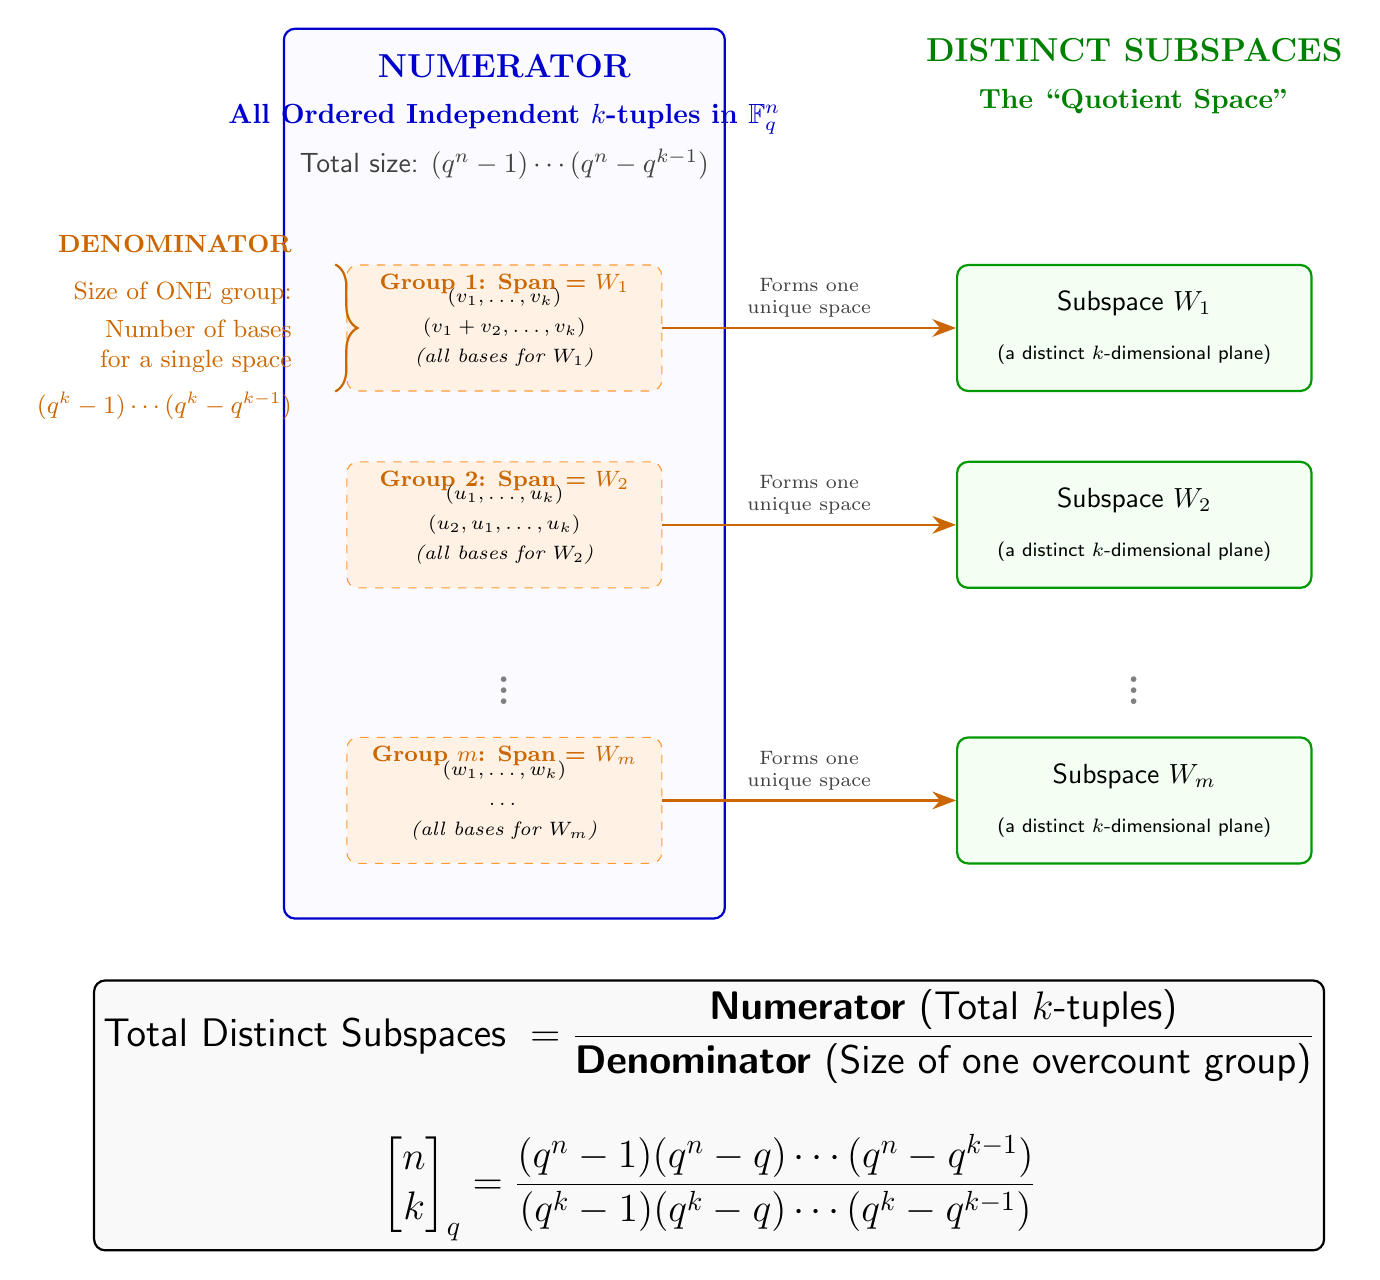
\begin{tikzpicture}[
		font=\sffamily,
		% Styles
		clusterbox/.style={draw=orange!80, fill=orange!10, dashed, rounded corners=4pt, minimum width=4cm, minimum height=1.6cm},
		subbox/.style={draw=green!60!black, fill=green!5, thick, rounded corners=4pt, minimum width=4.5cm, minimum height=1.6cm, align=center},
		arrow/.style={-{Stealth[length=3mm]}, thick, draw=orange!80!black}
		]
		
		% =========================================================
		% 1. LEFT SIDE: The big set (Numerator)
		% =========================================================
		\draw[draw=blue!80!black, fill=blue!2, thick, rounded corners] (-2.8, -5.5) rectangle (2.8, 5.8);
		
		\node[anchor=north, font=\bfseries\large, text=blue!80!black, align=center] at (0, 5.6) {NUMERATOR\\[1mm] \normalsize All Ordered Independent $k$-tuples in $\mathbb{F}_q^n$};
		\node[anchor=north, text=darkgray] at (0, 4.4) {Total size: $(q^n-1)\cdots(q^n-q^{k-1})$};
		
		% Clusters inside the big set (The equivalence classes)
		
		% Cluster 1
		\node[clusterbox] (C1) at (0, 2) {};
		\node[text=orange!80!black, font=\footnotesize\bfseries, anchor=north] at (C1.north) {Group 1: Span = $W_1$};
		\node[align=center, font=\scriptsize] at (C1.center) {$(v_1, \dots, v_k)$\\[1mm] $(v_1+v_2, \dots, v_k)$\\[1mm] \textit{(all bases for $W_1$)}};
		
		% Cluster 2
		\node[clusterbox] (C2) at (0, -0.5) {};
		\node[text=orange!80!black, font=\footnotesize\bfseries, anchor=north] at (C2.north) {Group 2: Span = $W_2$};
		\node[align=center, font=\scriptsize] at (C2.center) {$(u_1, \dots, u_k)$\\[1mm] $(u_2, u_1, \dots, u_k)$\\[1mm] \textit{(all bases for $W_2$)}};
		
		% Ellipsis
		\node[font=\Huge, text=gray] at (0, -2.5) {\vdots};
		
		% Cluster m
		\node[clusterbox] (Cm) at (0, -4) {};
		\node[text=orange!80!black, font=\footnotesize\bfseries, anchor=north] at (Cm.north) {Group $m$: Span = $W_m$};
		\node[align=center, font=\scriptsize] at (Cm.center) {$(w_1, \dots, w_k)$\\[1mm] $\dots$\\[1mm] \textit{(all bases for $W_m$)}};
		
		% =========================================================
		% 2. DENOMINATOR BRACE
		% =========================================================
		\draw[decorate, decoration={brace, amplitude=8pt, mirror}, thick, draw=orange!80!black] 
		([xshift=-4pt]C1.south west) -- ([xshift=-4pt]C1.north west) 
		node[midway, left=12pt, align=right, text=orange!80!black, font=\small] {
			\textbf{DENOMINATOR}\\[2mm] 
			Size of ONE group:\\[1mm]
			Number of bases\\
			for a single space\\[2mm]
			$(q^k-1)\cdots(q^k-q^{k-1})$
		};
		
		% =========================================================
		% 3. RIGHT SIDE: The Distinct Subspaces
		% =========================================================
		\node[anchor=south, font=\bfseries\large, text=green!50!black, align=center] at (8, 4.6) {DISTINCT SUBSPACES\\[1mm] \normalsize The ``Quotient Space''};
		
		% Subspace 1
		\node[subbox] (S1) at (8, 2) {Subspace $W_1$\\[2mm] \scriptsize (a distinct $k$-dimensional plane)};
		
		% Subspace 2
		\node[subbox] (S2) at (8, -0.5) {Subspace $W_2$\\[2mm] \scriptsize (a distinct $k$-dimensional plane)};
		
		% Ellipsis
		\node[font=\Huge, text=gray] at (8, -2.5) {\vdots};
		
		% Subspace m
		\node[subbox] (Sm) at (8, -4) {Subspace $W_m$\\[2mm] \scriptsize (a distinct $k$-dimensional plane)};
		
		% =========================================================
		% 4. MAPPINGS (Arrows from Groups to Distinct Spaces)
		% =========================================================
		\draw[arrow] (C1.east) -- (S1.west) node[midway, above, text=darkgray, font=\scriptsize, align=center] {Forms one\\unique space};
		\draw[arrow] (C2.east) -- (S2.west) node[midway, above, text=darkgray, font=\scriptsize, align=center] {Forms one\\unique space};
		\draw[arrow] (Cm.east) -- (Sm.west) node[midway, above, text=darkgray, font=\scriptsize, align=center] {Forms one\\unique space};
		
		% =========================================================
		% 5. FINAL FORMULA BLOCK
		% =========================================================
		\node[draw=black, thick, rounded corners, fill=gray!5, minimum width=11cm, minimum height=2cm, align=center] (Formula) at (2.6, -8) {
			\Large $\displaystyle \text{Total Distinct Subspaces } = \frac{\text{\textbf{Numerator}} \text{ (Total } k \text{-tuples)}}{\text{\textbf{Denominator}} \text{ (Size of one overcount group)}}$ \\[6mm]
			\Large $\displaystyle \begin{bmatrix} n \\ k \end{bmatrix}_q = \frac{(q^n-1)(q^n-q)\cdots(q^n-q^{k-1})}{(q^k-1)(q^k-q)\cdots(q^k-q^{k-1})}$
		};
		
	\end{tikzpicture}
\end{document}